\section[Tool]{Useful tools}

\subsection[Editor]{\cpp editor}

\begin{frame}[fragile]
  \frametitle{\cpp editor}
  \begin{block}{Choose it wisely}
    \begin{itemize}
    \item it can improve dramatically your efficiency by
      \begin{itemize}
      \item coloring the code for you to ``see'' the structure
      \item helping indenting properly
      \item allowing you to navigate easily in the source tree
      \item helping for compilation/debugging
      \end{itemize}
    \end{itemize}
  \end{block}
  \begin{block}{A few tools}
    \begin{description}
    \item[\href{http://www.microsoft.com/}{\beamergotobutton{Visual Studio}}]
      the Microsoft way
    \item[\href{https://code.visualstudio.com/}{\beamergotobutton{Visual Studio Code}}]
      more lightweight, open source and portable
    \item[\href{https://www.eclipse.org/}{\beamergotobutton{Eclipse}}]
      similar, also open source and portable
    \item[\href{http://www.gnu.org/software/emacs/}{\beamergotobutton{Emacs}} \href{https://www.vim.org/}{\beamergotobutton{Vim}}]
      the expert ways. Extremely powerful. \\
      They are to IDEs what latex is to PowerPoint
    \item[CLion, Code::Blocks, Atom, NetBeans, Sublime Text, ...]
    \end{description}
    Choosing one is mostly a matter of taste
  \end{block}
\end{frame}

\subsection[VCS]{Code management}

\begin{frame}[fragile]
  \frametitle{Code management tool}
  \begin{alertblock}{Please use one !}
    \begin{itemize}
    \item even locally
    \item even on a single file
    \item even if you are the only committer
    \end{itemize}
    It will soon save your day
  \end{alertblock}
  \begin{block}{A few tools}
    \begin{description}
    \item[\href{http://git-scm.com/}{\beamergotobutton{git}}]
      THE mainstream choice. Fast, light, easy to use
    \item[\href{http://mercurial.selenic.com/}{\beamergotobutton{mercurial}}]
      the alternative to git
    \item[\href{http://bazaar.canonical.com/en/}{\beamergotobutton{Bazaar}}]
      another alternative
    \item[svn]
      historical, not distributed - DO NOT USE
    \item[CVS]
      archeological, not distributed - DO NOT USE
    \end{description}
  \end{block}
\end{frame}

\begin{frame}[fragile]
  \frametitle{GIT crash course}
  \begin{minted}[gobble=4]{text}
    # git init myProject
    Initialized empty Git repository in myProject/.git/

    # vim file.cpp; vim file2.cpp
    # git add file.cpp file2.cpp
    # git commit -m "Committing first 2 files"
    [master (root-commit) c481716] Committing first 2 files
    ...

    # git log --oneline
    d725f2e Better STL test
    f24a6ce Reworked examples + added stl one
    bb54d15 implemented template part
    ...

    # git diff f24a6ce bb54d15
  \end{minted}
\end{frame}

\subsection[format]{Code formatting}

\begin{frame}[fragile]
\frametitle{clang-format}
\begin{block}{.clang-format}
	\begin{itemize}
		\item file describing your formatting preferences
		\item should be checked-in at the repository root (project wide)
		\item \mintinline{bash}{clang-format -style=LLVM -dump-config >} \\
		  \mintinline{bash}{.clang-format}
		\item adapt style options with help from: \url{https://clang.llvm.org/docs/ClangFormatStyleOptions.html}
	\end{itemize}
\end{block}
\begin{block}{Run clang-format}
	\begin{itemize}
		\item \mintinline{bash}{clang-format --style=LLVM -i <file.cpp>}
		\item \mintinline{bash}{clang-format -i <file.cpp>} (looks for .clang-format file)
		\item \mintinline{bash}{git clang-format} (formats local changes)
		\item \mintinline{bash}{git clang-format <ref>} (formats changes since git \textless{}ref\textgreater{})
		\item Some editors/IDEs find a .clang-format file and adapt
	\end{itemize}
\end{block}
\end{frame}

\begin{frame}[fragile]
\frametitle{clang-format}
\begin{alertblock}{Exercise Time}
	\begin{itemize}
		\item go to any example
		\item format code with: \mintinline{bash}{clang-format --style=GNU -i <file.cpp>}
		\item inspect changes, try \mintinline{bash}{git diff}
		\item revert changes using \mintinline{bash}{git checkout -- <file.cpp>}
		\item go to code directory and create a .clang-format file \\
		  \mintinline{bash}{clang-format -style=LLVM -dump-config >} \\
		  \mintinline{bash}{.clang-format}
		\item run \mintinline{bash}{clang-format -i */*.cpp}
		\item revert changes using \mintinline{bash}{git checkout .}
	\end{itemize}
\end{alertblock}
\end{frame}

\subsection[gcc]{The Compiling Chain}

\begin{frame}[fragile]
  \frametitlecpp[17]{The compiling chain}
  \center
  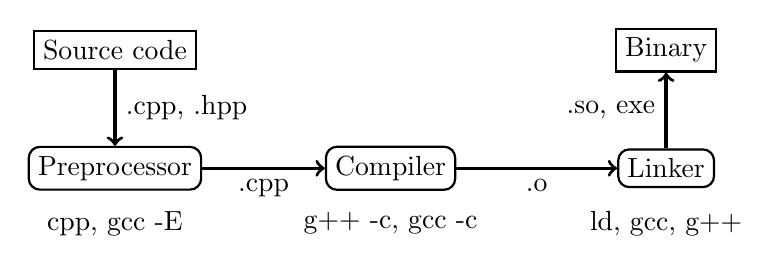
\begin{tikzpicture}
    \draw[thick] node (code) at(0,0) [rectangle,draw] {Source code}
                 node (cpp) at(0, -1.5cm) [rectangle,rounded corners,draw] {Preprocessor}
                 node (gcc) at(3.5cm,-1.5cm) [rectangle,rounded corners,draw] {Compiler}
                 node (ld) at(7cm,-1.5cm) [rectangle,rounded corners,draw] {Linker}
                 node (bin) at(7cm,0) [rectangle,draw] {Binary}
                 node at(0, -2.2cm) {cpp, gcc -E}
                 node at(3.5cm, -2.2cm) {g++ -c, gcc -c}
                 node at(7cm, -2.2cm) {ld, gcc, g++};
    \draw[very thick,->] (code) -- (cpp) node [midway,right] {.cpp, .hpp};
    \draw[very thick,->] (cpp) -- (gcc) node [midway,below] {.cpp};
    \draw[very thick,->] (gcc) -- (ld) node [midway,below] {.o};
    \draw[very thick,->] (ld) -- (bin) node [midway,left] {.so, exe};
  \end{tikzpicture}
  \begin{block}{The steps}
    \begin{description}
    \item[cpp]
        the preprocessor \\
        handles the \# directives (macros, includes) \\
        creates ``complete'' source code
    \item[g++]
        the compiler \\
        creates assembly code from \cpp code
    \item[ld]
        the linker \\
        links several binary files into libraries and executables
    \end{description}
  \end{block}
\end{frame}

\begin{frame}[fragile]
  \frametitle{Compilers}
  \begin{block}{Available tools}
    \begin{description}
    \item[\href{http://gcc.gnu.org/}{\beamergotobutton{gcc}}]
        the most common and most used\\
        free and open source
    \item[\href{http://clang.llvm.org/}{\beamergotobutton{clang}}]
        drop-in replacement of gcc \\
        slightly better error reporting \\
        free and open source, based on LLVM
    \item[\href{https://www.intel.com/content/www/us/en/developer/tools/oneapi/dpc-compiler.html\#gs.dyllp0}{\beamergotobutton{icc} \beamergotobutton{icx}}]
        the intel compilers, proprietary but now free \\
        optimized for Intel hardware \
        icc being replaced by icx, based on LLVM
    \item[\href{http://www.microsoft.com/}{\beamergotobutton{Visual \cpp}}]
      the Windows way
    \end{description}
  \end{block}
  \begin{alertblock}{My preferred choice today}
    \begin{itemize}
      \item \alert{gcc} as the de facto standard in HEP
      \item \hspace{0pt}\alert{clang} in parallel to catch more bugs
    \end{itemize}
  \end{alertblock}
\end{frame}

\begin{frame}[fragile]
  \frametitle{Useful compiler options (gcc/clang)}
  \begin{block}{Get more warnings}
    \begin{description}
      \item[-Wall -Wextra] the way to get all warnings
      \item[-Werror] the way to force yourself to look at warnings
    \end{description}
  \end{block}
  \begin{block}{Around optimization}
    \begin{description}
      \item[-g] add debug symbols
      \item[-O0, -O2] 0 = no optimization, -O2 = optimized
    \end{description}
  \end{block}
  \begin{block}{Compilation environment}
    \begin{description}
      \item[\texttt{-I} \textless{}path\textgreater] where to find header files
      \item[\texttt{-L} \textless{}path\textgreater] where to find libraries
      \item[\texttt{-l} \textless{}name\textgreater] link with libname.so
      \item[\texttt{-E / -c}] stop after preprocessing / compilation
    \end{description}
  \end{block}
\end{frame}

\begin{frame}[fragile]
  \frametitle{Makefiles}
  \begin{block}{Why to use them}
    \begin{itemize}
    \item an organized way of describing building steps
    \item avoids a lot of typing
    \end{itemize}
  \end{block}
  \begin{block}{Several implementations}
    \begin{itemize}
    \item raw Makefiles : suitable for small projects
    \item cmake : portable, the current best choice
    \item automake : GNU project solution
      \end{itemize}
  \end{block}
  \begin{minted}{makefile}
    test : test.cpp libpoly.so
        $(CXX) -Wall -Wextra -o $@ $^
    libpoly.so: Polygons.cpp
        $(CXX) -Wall -Wextra -shared -fPIC -o $@ $^
    clean:
        rm -f *o *so *~ test test.sol
  \end{minted}
\end{frame}

\begin{frame}[fragile]
  \frametitle{Compiler chain}
  \begin{alertblock}{Exercise Time}
    \begin{itemize}
    \item go to code/polymorphism
    \item preprocess Polygons.cpp (cpp or gcc -E -o output)
    \item compile Polygons.o and test.o (g++ -c -o output)
    \item use nm to check symbols in .o files
    \item look at the Makefile
    \item try make clean; make
    \item see linking stage using g++ -v
      \begin{itemize}
      \item just add a -v in the Makefile command for trypoly
      \item run make clean; make
      \item look at the collect 2 line, from the end up to ``-o trypoly''
      \end{itemize}
    \item see library dependencies with `ldd trypoly`
    \end{itemize}
  \end{alertblock}
\end{frame}

\subsection[gdb]{Debugging}

\begin{frame}[fragile]
  \frametitle{Debugging}
  \begin{alertblock}{The problem}
    \begin{itemize}
      \item everything compiles fine (no warning)
      \item but crashes at run time
      \item no error message, no clue
    \end{itemize}
  \end{alertblock}
  \pause
  \begin{block}{The solution : debuggers}
    \begin{itemize}
    \item dedicated program able to stop execution at any time
    \item and show you where you are and what you have
    \end{itemize}
  \end{block}
  \pause
  \begin{block}{Existing tools}
    \begin{description}
    \item[\href{http://www.sourceware.org/gdb/}{\beamergotobutton{gdb}}]
      THE main player
    \item[\href{http://lldb.llvm.org/}{\beamergotobutton{lldb}}]
      the debugger coming with clang, still young
    \item[\href{http://software.intel.com/en-us/articles/idb-linux}{\beamergotobutton{idb}}]
      the intel debugger, proprietary
    \end{description}
  \end{block}
\end{frame}

\begin{frame}[fragile]
  \frametitle{gdb crash course}
  \begin{block}{start gdb}
    \begin{itemize}
    \item gdb \textless{}program\textgreater
    \item gdb \textless{}program\textgreater \textless{}core file\textgreater
    \item gdb -{}-args \textless{}program\textgreater \textless{}program arguments\textgreater
    \end{itemize}
  \end{block}
  \begin{block}{inspect state}
    \begin{description}
    \item[bt] prints a backtrace
    \item[print \textless{}var\textgreater] prints current content of the variable
    \item[list] show code around current point
    \item[up/down] go up or down in call stack
    \end{description}
  \end{block}
  \begin{block}{breakpoints}
    \begin{description}
    \item[break \textless{}function\textgreater] puts a breakpoint on function entry
    \item[break \textless{}file\textgreater:\textless{}line\textgreater] puts a breakpoint on that line
    \end{description}
  \end{block}
\end{frame}

\begin{frame}[fragile]
  \frametitle{gdb}
  \begin{alertblock}{Exercise Time}
    \begin{itemize}
    \item go to code/debug
    \item compile, run, see the crash
    \item run it in gdb
    \item inspect backtrace, variables
    \item find problem and fix bug
    \item try stepping, breakpoints
    \item use -Wall -Wextra and see warning
    \end{itemize}
  \end{alertblock}
\end{frame}

\subsection[asan]{Address Sanitizer}

\begin{frame}[fragile]
  \frametitle{Address Sanitizer (asan)}
  \begin{block}{asan introduction}
    \begin{itemize}
    \item Compiler instrumentation supported by gcc and clang
    \item Program stops on invalid memory access, e.g.\
      \begin{itemize}
        \item Invalid read/write on heap and stack
        \item Double free/delete, use after free
        \item Buffer overflow on stack (few tools can do this)
        \item Only linux: memory leaks
      \end{itemize}
    \end{itemize}
  \end{block}
  \pause
  \begin{exampleblock}{Usage}
    \begin{itemize}
    \item Compile with \mintinline{bash}{-fsanitize=address -fno-omit-frame-pointer -g}
    \item With clang, add optionally: \texttt{-fsanitize-address-use-after-return=always -fsanitize-address-use-after-scope}
    \item Link with \mintinline{bash}{-fsanitize=address}
    \item Run the program
    \end{itemize}
  \end{exampleblock}
\end{frame}

\begin{frame}[fragile]
  \frametitle{Address Sanitizer (asan)}
  \begin{block}{How it works}
    \begin{itemize}
      \item Compiler adds run-time checks ($\sim$2x slow down)
      \item \mintinline{cpp}{IsPoisoned(address)} looks up state of address in asan's ``shadow memory''
      \item Shadow memory: memory where 1 shadow byte tracks state of 8 application bytes (state = accessible, poisoned, \ldots)
      \item Functions that deal with memory (\mintinline{cpp}{new() / delete()} / strings / ...) update entries in shadow memory when called
    \end{itemize}
  \end{block}
  \begin{exampleblock}{asan instrumentation (mock code)}
    \begin{overprint}
      \onslide<1>
      \vfill
      \begin{cppcode*}{gobble=4}
        int i = *address;
      \end{cppcode*}
      \onslide<2->
      \vfill
      \begin{cppcode*}{gobble=4}
        if (IsPoisoned(address)) {
          ReportError(address, kAccessSize, kIsWrite);
        }
        int i = *address;
      \end{cppcode*}
    \end{overprint}
  \end{exampleblock}
\end{frame}


\begin{frame}[fragile]
  \begin{block}{asan red zones}
    \begin{itemize}
      \item If adjacent data blocks are owned by the process, the operating system will allow an access
      \item<2> asan surrounds blocks of memory by poisoned red zones
      \item<2> Program stops when accessing a red zone
    \end{itemize}
  \end{block}
  \begin{exampleblock}{Illegal access (not detected without asan)}
    \begin{multicols}{2}
      \begin{overprint}
        \onslide<1>
        \begin{minted}{cpp}
 void foo() {
   char a[8];
   char b[8];
   a[8] = '1';
 }
        \end{minted}
        \onslide<2>
        \begin{minted}{diff}
 void foo() {
+  char redzone1[32];
   char a[8];
+  char redzone2[24];
   char b[8];
+  char redzone3[24];
+  // <poison redzones>
   a[8] = '1';
+  // <unpoison redzones>
 }
        \end{minted}
      \end{overprint}
      \columnbreak
      \begin{tikzpicture}
        \clip (0,0) rectangle (6cm, 3cm);
        \memorystack[word size=4,nb blocks=4]
        \onslide<1>{
          \draw[fill=green!70,opacity=0.5] (0.,0.*\stacksizey) rectangle (\stacksizex/4.,1.*\stacksizey) node[midway]{\footnotesize a[0-7]};
          \draw[fill=orange,opacity=0.5] (\stacksizex/4.,0.*\stacksizey) rectangle (\stacksizex/2.,1.*\stacksizey) node[midway]{\footnotesize b[0-7]};
        }
        \memorygoto{2}
        \onslide<2->{
          \draw[fill=red!70,opacity=0.5] (0.,0.*\stacksizey) rectangle (\stacksizex,1.*\stacksizey) node[midway]{redzone1};
          \memorypush{a[0-7]}
          \draw[fill=red!70,opacity=0.5] (0.+\stacksizex/4.,1.*\stacksizey) rectangle (\stacksizex,2.*\stacksizey) node[midway]{redzone2};
          \memorypush{b[0-7]}
          \draw[fill=red!70,opacity=0.5] (0.+\stacksizex/4.,2.*\stacksizey) rectangle (\stacksizex,3.*\stacksizey) node[midway]{redzone3};
        }
      \end{tikzpicture}
    \end{multicols}
    \vspace{1mm}
  \end{exampleblock}
\end{frame}

\begin{frame}[fragile]
  \vspace{-1\baselineskip}
  \begin{columns}
    \column{\textwidth+1cm}
    \scriptsize
    \begin{Verbatim}[commandchars=\\\{\}]
    \ttfamily
\textcolor{green}{==34015==ERROR: AddressSanitizer: stack-buffer-overflow on address 0x7ffee93ed968 at pc 0x000106812df4 bp 0x7ffee93ed930 sp 0x7ffee93ed928}
\textcolor{blue}{WRITE of size 1 at 0x7ffee93ed968 thread T0}
    #0 0x106812df3 in foo() asan.cpp:4
    #1 0x106812ed8 in main asan.cpp:9
    #2 0x7fff6d3923d4 in start (libdyld.dylib:x86_64+0x163d4)

\textcolor{green}{Address 0x7ffee93ed968 is located in stack of thread T0 at offset 40 in frame}
    #0 0x106812cdf in foo() asan.cpp:1

  This frame has 2 object(s):
    [32, 40) 'a' (line 2) \textcolor{green}{<== Memory access at offset 40 overflows this variable}
    [64, 72) 'b' (line 3)
Shadow bytes around the buggy address:
=>0x1fffdd27db20: 00 00 00 00 00 00 00 00 \textcolor{red}{f1 f1 f1 f1} 00[\textcolor{red}{f2}]\textcolor{red}{f2 f2}
  0x1fffdd27db30: 00 \textcolor{red}{f3 f3 f3} 00 00 00 00 00 00 00 00 00 00 00 00
  0x1fffdd27db40: 00 00 00 00 00 00 00 00 00 00 00 00 00 00 00 00
  0x1fffdd27db50: 00 00 00 00 00 00 00 00 00 00 00 00 00 00 00 00
Shadow byte legend (one shadow byte represents 8 application bytes):
  Addressable:           00
  Partially addressable: 01 02 03 04 05 06 07
  Heap left redzone:       \textcolor{red}{fa}
  Freed heap region:       \textcolor{pink}{fd}
  Stack left redzone:      \textcolor{red}{f1}
  Stack mid redzone:       \textcolor{red}{f2}
  Stack right redzone:     \textcolor{red}{f3}
  Stack after return:      \textcolor{pink}{f5}
    \end{Verbatim}
  \end{columns}
\end{frame}

\begin{frame}[fragile]
  \begin{columns}
    \column{\textwidth+1cm}
    \begin{block}{Finding memory leaks with asan}
      \begin{itemize}
        \item On linux, asan can display memory leaks
        \item Start executable with \mintinline{bash}{ASAN_OPTIONS=detect_leaks=1 ./myProgram}
      \end{itemize}
    \end{block}
    \scriptsize
    \begin{Verbatim}[commandchars=\\\{\}]
    \ttfamily
\textcolor{red}{==113262==ERROR: LeakSanitizer: detected memory leaks}

\textcolor{blue}{Direct leak of 32 byte(s) in 1 object(s) allocated from:}
  #0 0x7f2671201647 in operator new(unsigned long) /build/dkonst/WORK/build/contrib/gcc-10.1.0/src/gcc/10.1.0/libsanitizer/asan/asan_new_delete.cpp:99
  #1 0x4033c7 in memoryLeak[abi:cxx11]() /afs/cern.ch/user/s/shageboe/asan.cpp:33
  #2 0x403633 in main /afs/cern.ch/user/s/shageboe/asan.cpp:40
  #3 0x7f2670a15492 in __libc_start_main (/lib64/libc.so.6+0x23492)

\textcolor{blue}{Indirect leak of 22 byte(s) in 1 object(s) allocated from:}
  #0 0x7f2671201647 in operator new(unsigned long) /build/dkonst/WORK/build/contrib/gcc-10.1.0/src/gcc/10.1.0/libsanitizer/asan/asan_new_delete.cpp:99
  #1 0x403846 in void std::__cxx11::basic_string<char, std::char_traits<char>, std::allocator<char> >::_M_construct<char const*>(char const*, char const*, std::forward_iterator_tag) /cvmfs/sft.cern.ch/lcg/releases/gcc/10.1.0.c82-6f386/x86_64-centos8/include/c++/10.1.0/bits/basic_string.tcc:219
  #2 0x4033f4 in std::__cxx11::basic_string<char, std::char_traits<char>, std::allocator<char> >::basic_string<std::allocator<char> >(char const*, std::allocator<char> const&) /cvmfs/sft.cern.ch/lcg/releases/gcc/10.1.0.c82-6f386/x86_64-centos8/include/c++/10.1.0/bits/basic_string.h:247
  #3 0x4033f4 in memoryLeak[abi:cxx11]() /afs/cern.ch/user/s/shageboe/asan.cpp:33
  #4 0x403633 in main /afs/cern.ch/user/s/shageboe/asan.cpp:40
  #5 0x7f2670a15492 in __libc_start_main (/lib64/libc.so.6+0x23492)

SUMMARY: AddressSanitizer: 54 byte(s) leaked in 2 allocation(s).
    \end{Verbatim}
  \end{columns}
\end{frame}

\begin{frame}[fragile]
  \frametitle{Address sanitizer (asan)}
  \begin{block}{Wrap up}
    \begin{itemize}
      \item If a program crashes, run it with asan
      \item Asan should be part of every \cpp{} CI
      \item It will also find bugs that by luck didn't crash the program
      \item It doesn't generate false positives
    \end{itemize}
  \end{block}

  \begin{exampleblock}{More info}
    \begin{itemize}
      \item \url{https://github.com/google/sanitizers/wiki/AddressSanitizer}
      \item Compile with asan, and start executable using \mintinline{bash}{ASAN_OPTIONS=help=1 <executable>}
    \end{itemize}
  \end{exampleblock}
\end{frame}

\begin{frame}[fragile]
  \frametitle{Address sanitizer (asan)}
  \begin{alertblock}{Hands on}
    \begin{itemize}
      \item Go to \texttt{code/asan}
      \item Compile and run the program \texttt{./asan}
      \item There are two bugs and one memory leak. Use asan to trace them down.
    \end{itemize}
  \end{alertblock}

\end{frame}


\subsection[valgrind]{The Valgrind family}

\begin{frame}[fragile]
  \frametitle{The valgrind family}
  \begin{block}{Valgrind fundamentals}
    \begin{itemize}
    \item valgrind is a framework for different tools
    \item a processor simulator allowing checks in between instructions
    \item slow (10-50 times slower than normal execution)
    \item easy to use : ``valgrind \textless{}your executable\textgreater''
      \begin{itemize}
      \item no recompilation
      \item better with -g -O0, but not strictly needed
      \end{itemize}
    \item it is free and open source
    \end{itemize}
  \end{block}
  \pause
  \begin{block}{Main tools}
    \begin{description}
      \item[memcheck] a memory checker (default tool) and leak detector
      \item[callgrind] a call graph builder
      \item[helgrind] a race condition detector
    \end{description}
  \end{block}
\end{frame}

\begin{frame}[fragile]
  \frametitle{memcheck}
  \begin{block}{}
    \begin{itemize}
      \item keeps track of all memory allocations and deallocations
      \item is able to detect accesses to unallocated memory
      \item and even tell you when it was deallocated if it was
      \item or what is the closest array in case of overflow
      \item is able to list still allocated memory when program exits\\
        (memory leaks detection)
    \end{itemize}
  \end{block}
\end{frame}

\begin{frame}[fragile]
  \frametitle{valgrind}
  \begin{alertblock}{Exercise Time}
    \begin{itemize}
    \item go to code/valgrind
    \item compile, run, it should work
    \item run with valgrind, see the problem
    \item fix the problem
      \vspace{.3cm}
    \item go back to the code/debug exercise
    \item check it with valgrind
    \item analyze the issue, see that the variance was biaised
    \item fix the issue
    \end{itemize}
  \end{alertblock}
\end{frame}

\begin{frame}[fragile]
  \frametitle{memcheck}
  \begin{alertblock}{Exercise Time}
    \begin{itemize}
    \item go to code/memcheck
    \item compile, run, it should work
    \item run with valgrind, see LEAK summary
    \item run with -{}-leak-check=full to get details
    \item analyze and correct it
    \end{itemize}
  \end{alertblock}
\end{frame}

\begin{frame}[fragile]
  \frametitle{callgrind and kcachegrind}
  \begin{block}{callgrind}
    \begin{itemize}
      \item keeps track of all function calls
      \item and time spent in each function
      \item build statistics on calls, CPU usages and more
      \item outputs flat statistics file, quite unreadable
    \end{itemize}
  \end{block}
  \begin{block}{kcachegrind}
    \begin{itemize}
      \item a gui exploiting statistics built by callgrind
      \item able to browse graphically the program calls
      \item able to ``graph'' CPU usage on the program structure
    \end{itemize}
  \end{block}
\end{frame}

\begin{frame}[fragile]
  \frametitle{callgrind}
  \begin{alertblock}{Exercise Time}
    \begin{itemize}
    \item go to code/callgrind
    \item compile, run, it will be slow
    \item change nb iterations to 20
    \item run with valgrind -{}-tool=callgrind
    \item look at output with kcachegrind
    \item change fibo call to fibo2
    \item observe the change in kcachegrind
    \end{itemize}
  \end{alertblock}
\end{frame}

\begin{frame}[fragile]
  \frametitle{helgrind}
  \begin{block}{}
    \begin{itemize}
      \item keeps track of all pthreads activity
      \item in particular keeps track of all mutexes
      \item builds a graph of dependencies of the different actions
      \item works on the resulting graph to detect:
        \begin{itemize}
        \item possible dead locks
        \item possible data races
        \end{itemize}
    \end{itemize}
  \end{block}
  \pause
  \begin{alertblock}{}
    Note the ``possible''. It finds future problems !
  \end{alertblock}
\end{frame}

\begin{frame}[fragile]
  \frametitle{helgrind}
  \begin{alertblock}{Exercise Time}
    \begin{itemize}
    \item go to code/helgrind
    \item compile, run
    \item check it with valgrind. You may see strange behavior \\
      or it will be perfectly fine
    \item check it with valgrind -{}-tool=helgrind
    \item understand issue and fix
    \end{itemize}
  \end{alertblock}
\end{frame}

\subsection[static]{Static code analysis}

\begin{frame}[fragile]
  \frametitle{Static analysis}
  \begin{alertblock}{The problem}
    \begin{itemize}
    \item all the tools discussed so far work on binaries
    \item they analyze the code being run
    \item so there is a coverage problem (e.g. for error cases)
    \end{itemize}
  \end{alertblock}
  \pause
  \begin{block}{A (partial) solution : analyzing the source code}
    \begin{itemize}
    \item build a graph of dependencies of the calls
    \item use graph tools to detect potential memory corruptions,
      memory leaks or missing initializations
    \end{itemize}
  \end{block}
  \pause
  \begin{block}{Existing tools}
    \begin{description}
    \item[\href{http://www.coverity.com/}{\beamergotobutton{Coverity}}]
      proprietary tool, the most complete
    \item[\href{http://cppcheck.sourceforge.net/}{\beamergotobutton{cppcheck}}]
      free and opensource, but less complete
    \item[\href{https://clang.llvm.org/extra/clang-tidy/}{\beamergotobutton{clang-tidy}}]
      clang-based ``linter'', includes clang static analyzer
    \end{description}
  \end{block}
\end{frame}

\begin{frame}[fragile]
  \frametitle{cppcheck}
  \begin{alertblock}{Exercise Time}
    \begin{itemize}
    \item go to code/cppcheck
    \item compile, run, see that it works
    \item use valgrind : no issue
    \item use cppcheck, see the problem
    \item analyze the issue, and fix it
    \item bonus : understand why valgrind did not complain \\
      and how the standard deviation could be biased \\
      hint : use gdb and check addresses of v and diffs
    \end{itemize}
  \end{alertblock}
\end{frame}

\begin{frame}[fragile]
  \frametitle{clang-tidy}
  \begin{block}{Documentation and supported checks}
    \begin{itemize}
      \item \url{https://clang.llvm.org/extra/clang-tidy/}
    \end{itemize}
  \end{block}
  \begin{block}{Run clang-tidy}
    \begin{itemize}
      \item \mintinline{bash}{clang-tidy <file.cpp> -checks=...}
      \item \mintinline{bash}{clang-tidy <file.cpp>} (checks from .clang-tidy file)
      \item \mintinline{bash}{clang-tidy <file.cpp> --fix} (applies fixes)

    \end{itemize}
  \end{block}
  \begin{block}{Compilation flags}
    \begin{itemize}
      \item clang-tidy needs to know exactly how your program is built
      \item \mintinline{bash}{clang-tidy ... -- <all compiler flags>}
    \end{itemize}
  \end{block}
  \begin{block}{.clang-tidy file}
    \begin{itemize}
      \item describes which checks to run
      \item usually checked in at repository root
    \end{itemize}
  \end{block}
\end{frame}

\begin{frame}[fragile]
  \begin{block}{Automatically collecting compilation flags}
    \begin{itemize}
      \item clang-tidy looks for a file called compile\_commands.json
      \item contains the exact build flags for each .cpp file
      \item generate with CMake: \\
        \mintinline{bash}{cmake -DCMAKE_EXPORT_COMPILE_COMMANDS=ON ...}
      \item for Makefiles try \href{https://github.com/rizsotto/Bear}{\beamergotobutton{Bear}}
      \item allows to run clang-tidy in bulk on all files:
      \begin{itemize}
        \item \mintinline{bash}{run-clang-tidy -checks ...}
        \item \mintinline{bash}{run-clang-tidy} (checks from .clang-tidy)
        \item \mintinline{bash}{run-clang-tidy -fix} (applies fixes)
      \end{itemize}
    \end{itemize}
  \end{block}
\end{frame}

\begin{frame}[fragile]
  \frametitle{clang-tidy}
  \begin{alertblock}{Exercise Time}
    \begin{itemize}
      \item go to any example which compiles (e.g. code/cppcheck)
      \item \mintinline{bash}{mkdir build && cd build}
      \item \mintinline{bash}{cmake -DCMAKE_EXPORT_COMPILE_COMMANDS=ON ..}
      \item \mintinline{bash}{clang-tidy <../file.cpp> -checks=*}
      \item inspect output
      \item run with \mintinline{bash}{--fix} flag
      \item revert changes using \mintinline{bash}{git checkout <../file.cpp>}
    \end{itemize}
  \end{alertblock}
\end{frame}
